\documentclass{beamer}
\usepackage[utf8]{inputenc}

\usetheme{Madrid}
\usecolortheme{default}
\usepackage{amsmath,amssymb,amsfonts,amsthm}
\usepackage{txfonts}
\usepackage{tkz-euclide}
\usepackage{listings}
\usepackage{adjustbox}
\usepackage{array}
\usepackage{tabularx}
\usepackage{gvv}
\usepackage{lmodern}
\usepackage{circuitikz}
\usepackage{tikz}
\usepackage{graphicx}

\setbeamertemplate{page number in head/foot}[totalframenumber]

\usepackage{tcolorbox}
\tcbuselibrary{minted,breakable,xparse,skins}



\definecolor{bg}{gray}{0.95}
\DeclareTCBListing{mintedbox}{O{}m!O{}}{%
	breakable=true,
	listing engine=minted,
	listing only,
	minted language=#2,
	minted style=default,
	minted options={%
		linenos,
		gobble=0,
		breaklines=true,
		breakafter=,,
		fontsize=\small,
		numbersep=8pt,
		#1},
	boxsep=0pt,
	left skip=0pt,
	right skip=0pt,
	left=25pt,
	right=0pt,
	top=3pt,
	bottom=3pt,
	arc=5pt,
	leftrule=0pt,
	rightrule=0pt,
	bottomrule=2pt,
	toprule=2pt,
	colback=bg,
	colframe=orange!70,
	enhanced,
	overlay={%
		\begin{tcbclipinterior}
			\fill[orange!20!white] (frame.south west) rectangle ([xshift=20pt]frame.north west);
	\end{tcbclipinterior}},
	#3,
}
\lstset{
	language=C,
	basicstyle=\ttfamily\small,
	keywordstyle=\color{blue},
	stringstyle=\color{orange},
	commentstyle=\color{green!60!black},
	numbers=left,
	numberstyle=\tiny\color{gray},
	breaklines=true,
	showstringspaces=false,
}
%------------------------------------------------------------
%This block of code defines the information to appear in the
%Title page
\title %optional
{4.11.14}
\date{}
%\subtitle{A short story}

\author % (optional)
{M Chanakya Srinivas- EE25BTECH11036}




\begin{document}


\frame{\titlepage}



\begin{frame}{Problem}
Find \(\lambda\) so that
\[
\frac{x-5}{5\lambda+2}=\frac{2-y}{5}=\frac{1-z}{-1},\qquad
\frac{x}{1}=\frac{y+\tfrac12}{2\lambda}=\frac{z-1}{3}
\]
are perpendicular; determine intersection condition.
\end{frame}

\begin{frame}{Vector form \& perpendicularity}
Choose
\[
\vec{A}_1=\myvec{5\\2\\1},\ \vec{m}_1=\myvec{5\lambda+2\\-5\\1},\qquad
\vec{A}_2=\myvec{0\\-\tfrac12\\1},\ \vec{m}_2=\myvec{1\\2\lambda\\3}.
\]
Compute
\[
\vec{m}_1^\top\vec{m}_2 = (5\lambda+2)-10\lambda+3 = -5\lambda+5.
\]
Hence \(\boxed{\lambda=1}\) for perpendicular directions.
\end{frame}

\begin{frame}{Set up augmented matrix}
Intersection needs \(\kappa_1,\kappa_2\) solving
\(\kappa_1\vec{m}_1-\kappa_2\vec{m}_2=\vec{A}_2-\vec{A}_1\).
Write the augmented matrix:
\[
\mathcal{M}_0 =
\left[\begin{array}{cc|c}
5\lambda+2 & -1 & -5 \\[2pt]
-5 & -2\lambda & -\tfrac{5}{2} \\[2pt]
1 & -3 & 0
\end{array}\right].
\]
We reduce \(\mathcal{M}_0\) to RREF using explicit row operations.
\end{frame}

\begin{frame}{RREF — Step 1 (swap)}
Swap \(R_1\leftrightarrow R_3\):
\[
\mathcal{M}_1 =
\left[\begin{array}{cc|c}
1 & -3 & 0 \\
-5 & -2\lambda & -\tfrac{5}{2} \\
5\lambda+2 & -1 & -5
\end{array}\right].
\]
\end{frame}

\begin{frame}{RREF — Step 2 (eliminate col 1)}
Eliminate first column using \(R_1\):
\[
R_2\leftarrow R_2+5R_1,\qquad R_3\leftarrow R_3-(5\lambda+2)R_1,
\]
giving
\[
\mathcal{M}_2 =
\left[\begin{array}{cc|c}
1 & -3 & 0 \\
0 & -2\lambda-15 & -\tfrac{5}{2} \\
0 & 15\lambda+5 & -5
\end{array}\right].
\]
\end{frame}

\begin{frame}{RREF — Step 3 (scale R2 and eliminate)}
Scale \(R_2\) by \(1/(-2\lambda-15)\) (if nonzero) and eliminate column~2:
\[
R_2\leftarrow \frac{1}{-2\lambda-15}R_2,\quad
R_1\leftarrow R_1+3R_2,\quad
R_3\leftarrow R_3-(15\lambda+5)R_2.
\]
Resulting matrix has form
\[
\mathcal{M}_4 =
\left[\begin{array}{cc|c}
1 & 0 & * \\
0 & 1 & * \\
0 & 0 & r
\end{array}\right],
\]
where \(r\) is the residual determining consistency.
\end{frame}

\begin{frame}{Consistency condition (RREF read-off)}
From \(\mathcal{M}_2\) the two scalar rows give
\[
(-2\lambda-15)\kappa_2=-\tfrac{5}{2},\qquad (15\lambda+5)\kappa_2=-5.
\]
So
\[
\kappa_2=\frac{5}{30+4\lambda} \quad\text{and}\quad
\kappa_2=-\frac{1}{3\lambda+1}.
\]
Equate them:
\[
-\frac{1}{3\lambda+1}=\frac{5}{30+4\lambda}
\]
which yields \(\boxed{\lambda=-\tfrac{35}{19}}\) (intersection case).
\end{frame}

\begin{frame}{Check \(\lambda=1\)}
At \(\lambda=1\) the two equations give
\[
\kappa_2=\tfrac{5}{34}\quad\text{and}\quad \kappa_2=-\tfrac{1}{4},
\]
a contradiction. Thus augmented system inconsistent \(\Rightarrow\) lines are skew for \(\lambda=1\).
\end{frame}

\begin{frame}{Summary}
\begin{itemize}
\item \(\lambda=1\) : direction vectors perpendicular; lines do not intersect (skew).
\item \(\lambda=-\dfrac{35}{19}\) : RREF consistent; lines intersect (not perpendicular).
\end{itemize}
\end{frame}


\begin{frame}[fragile]{C code}
\begin{lstlisting}
    #include <math.h>
// Return lambda for which the two lines are perpendicular.
double perpendicular_lambda(void) {
    return 1.0;
}
// Return lambda for which the two lines intersect.
double intersection_lambda(void) {
    return -35.0/19.0;
}
// For a given lambda, check whether the two lines intersect.
// Writes s (parameter of line2) and t (parameter of line1) to the output pointers.
// Returns 1 if intersection exists (within tolerance), otherwise 0.
int lines_intersection_params(double lambda, double *s_out, double *t_out) {
    const double EPS = 1e-9;
    double denom1 = 1.0 - 3.0*(5.0*lambda + 2.0);
    if (fabs(denom1) < EPS) return 0;
     \end{lstlisting}
\end{frame}
    \begin{frame}[fragile]{C code}
\begin{lstlisting}
    double s1 = 5.0/denom1;
    double denom2 = 30.0 + 4.0*lambda;
    if (fabs(denom2) < EPS) return 0;
    double s2 = 5.0/denom2;
    if (fabs(s1 - s2) > 1e-6) return 0;
    double s = 0.5*(s1 + s2);
    double t = 3.0*s;
    if (s_out) *s_out = s;
    if (t_out) *t_out = t;
    return 1;
}
 \end{lstlisting}
\end{frame}
    \begin{frame}[fragile]{Python code through shared output}
\begin{lstlisting}
import ctypes
from fractions import Fraction
import numpy as np
import matplotlib.pyplot as plt
from mpl_toolkits.mplot3d import Axes3D

# Load shared library
lib = ctypes.CDLL('./liblines.so')
lib.perpendicular_lambda.restype = ctypes.c_double
lib.intersection_lambda.restype = ctypes.c_double
lib.lines_intersection_params.restype = ctypes.c_int
lib.lines_intersection_params.argtypes = [
    ctypes.c_double,
    ctypes.POINTER(ctypes.c_double),
    ctypes.POINTER(ctypes.c_double)
]
\end{lstlisting}
\end{frame}
  \begin{frame}[fragile]{Python code through shared output}
\begin{lstlisting}
# 1. Get lambdas
lam_perp = lib.perpendicular_lambda()
lam_inter = lib.intersection_lambda()

print(f"Lambda for perpendicular lines: {lam_perp} = {Fraction(lam_perp).limit_denominator()}")
print(f"Lambda for intersection: {lam_inter} = {Fraction(lam_inter).limit_denominator()}")

# 2. Check intersection at perpendicular lambda
s1 = ctypes.c_double()
t1 = ctypes.c_double()
intersects_perp = lib.lines_intersection_params(lam_perp, ctypes.byref(s1), ctypes.byref(t1))

# 3. Check intersection at intersection lambda
s2 = ctypes.c_double()
t2 = ctypes.c_double()
intersects = lib.lines_intersection_params(lam_inter, ctypes.byref(s2), ctypes.byref(t2))
\end{lstlisting}
\end{frame}
  \begin{frame}[fragile]{Python code through shared output}
\begin{lstlisting}
if intersects_perp:
    print("Lines intersect when perpendicular.")
else:
    print("❌ Lines do NOT intersect when they are perpendicular.")

if intersects:
    print("✅ Lines intersect when λ =", lam_inter)
    print("Intersection parameters: s =", s2.value, ", t =", t2.value)
    inter_point = np.array([
        s2.value,
        -0.5 + 2*lam_inter*s2.value,
        1 + 3*s2.value
    ])
    print("Intersection point:", inter_point)
else:
    inter_point = None
    print("❌ Lines do NOT intersect for intersection λ.")
\end{lstlisting}
\end{frame}
  \begin{frame}[fragile]{Python code through shared output}
\begin{lstlisting}
# 4. Plot
t_vals = np.linspace(-2, 2, 100)
x1 = 5 + (5*lam_inter + 2)*t_vals
y1 = 2 - 5*t_vals
z1 = 1 + t_vals

s_vals = np.linspace(-2, 2, 100)
x2 = s_vals
y2 = -0.5 + 2*lam_inter*s_vals
z2 = 1 + 3*s_vals

fig = plt.figure(figsize=(10, 8))
ax = fig.add_subplot(111, projection='3d')

# Plot lines
ax.plot(x1, y1, z1, label="Line 1", color='blue', linewidth=2)
ax.plot(x2, y2, z2, label="Line 2", color='red', linewidth=2)
\end{lstlisting}
\end{frame}
  \begin{frame}[fragile]{Python code through shared output}
\begin{lstlisting}
# Plot intersection
if inter_point is not None:
    ax.scatter(*inter_point, color='green', s=80, edgecolors='black', label="Intersection Point")
    ax.text(*inter_point + 0.3, 
            f"({inter_point[0]:.2f}, {inter_point[1]:.2f}, {inter_point[2]:.2f})",
            fontsize=10, color='green')
\end{lstlisting}
\end{frame}
  \begin{frame}[fragile]{Python code through shared output}
\begin{lstlisting}
# Labels and legend
ax.set_xlabel("X Axis", fontsize=12)
ax.set_ylabel("Y Axis", fontsize=12)
ax.set_zlabel("Z Axis", fontsize=12)
ax.set_title("3D Plot: Intersection of Two Lines", fontsize=14)
ax.legend()
ax.grid(True)
ax.view_init(elev=25, azim=135)

plt.tight_layout()
plt.show()

 \end{lstlisting}
\end{frame}
  \begin{frame}[fragile]{Only Python code}
\begin{lstlisting}
import numpy as np
import matplotlib.pyplot as plt

# Local imports (assuming these scripts are available and in PYTHONPATH)
from line.funcs import *
from triangle.funcs import *
from conics.funcs import circ_gen

# Given intersection parameter lambda (from your C-types code or calculation)
lam = -35/19  # approx -1.8421

# Calculate intersection parameters s and t for the lines
# The two parametric lines from your problem:
 \end{lstlisting}
\end{frame}
  \begin{frame}[fragile]{Only Python code}
\begin{lstlisting}
# Line 1:
# x = 5 + (5*lam + 2)*t
# y = 2 - 5*t
# z = 1 + t

# Line 2:
# x = s
# y = -0.5 + 2*lam*s
# z = 1 + 3*s

# We want to find s, t such that both lines intersect

# From parametric equality:
# 5 + (5*lam + 2)*t = s      ...(1)
# 2 - 5*t = -0.5 + 2*lam*s   ...(2)
# 1 + t = 1 + 3*s            ...(3)

# Solve (3):
# t = 3*s
 \end{lstlisting}
\end{frame}
  \begin{frame}[fragile]{Only Python code}
\begin{lstlisting}
# Substitute into (1):
# 5 + (5*lam + 2)*3*s = s
# 5 + 3*(5*lam + 2)*s = s
# 5 = s - 3*(5*lam + 2)*s = s*(1 - 3*(5*lam + 2))
# s = 5 / (1 - 3*(5*lam + 2))

denom = 1 - 3*(5*lam + 2)
s = 5 / denom

# Then t = 3*s
t = 3*s

# Calculate intersection point from line 2 (or line 1)
inter_point = np.array([
    s,
    -0.5 + 2*lam*s,
    1 + 3*s
])
 \end{lstlisting}
\end{frame}
  \begin{frame}[fragile]{Only Python code}
\begin{lstlisting}
print(f"Intersection parameters: s = {s:.5f}, t = {t:.5f}")
print(f"Intersection Point: ({inter_point[0]:.5f}, {inter_point[1]:.5f}, {inter_point[2]:.5f})")

# Define parametric lines for plotting near intersection point

def line1(t_vals):
    x = 5 + (5*lam + 2)*t_vals
    y = 2 - 5*t_vals
    z = 1 + t_vals
    return x, y, z

def line2(s_vals):
    x = s_vals
    y = -0.5 + 2*lam*s_vals
    z = 1 + 3*s_vals
    return x, y, z
 \end{lstlisting}
\end{frame}
  \begin{frame}[fragile]{Only Python code}
\begin{lstlisting}
# Plot ranges close to intersection
t_vals = np.linspace(t - 1, t + 1, 100)
s_vals = np.linspace(s - 1, s + 1, 100)

x1, y1, z1 = line1(t_vals)
x2, y2, z2 = line2(s_vals)

# Plotting
fig = plt.figure(figsize=(10, 8))
ax = fig.add_subplot(111, projection='3d')

ax.plot(x1, y1, z1, label='Line 1', color='blue', linewidth=2)
ax.plot(x2, y2, z2, label='Line 2', color='red', linewidth=2)

# Mark intersection
ax.scatter(*inter_point, color='green', s=80, label='Intersection Point')
 \end{lstlisting}
\end{frame}
  \begin{frame}[fragile]{Only Python code}
\begin{lstlisting}
# Annotate intersection point
ax.text(inter_point[0], inter_point[1], inter_point[2],
        f"A\n({inter_point[0]:.2f}, {inter_point[1]:.2f}, {inter_point[2]:.2f})",
        color='green', fontsize=12, ha='center', va='bottom')

# Axis labels and title
ax.set_xlabel("X axis", fontsize=12)
ax.set_ylabel("Y axis", fontsize=12)
ax.set_zlabel("Z axis", fontsize=12)
ax.set_title("3D Plot of Two Lines and their Intersection", fontsize=14)

ax.legend()
ax.grid(True)
ax.view_init(elev=20, azim=45)

plt.tight_layout()
plt.show()

 \end{lstlisting}
\end{frame}
\begin{frame}{PLOTS}
    \begin{figure}
        \centering
        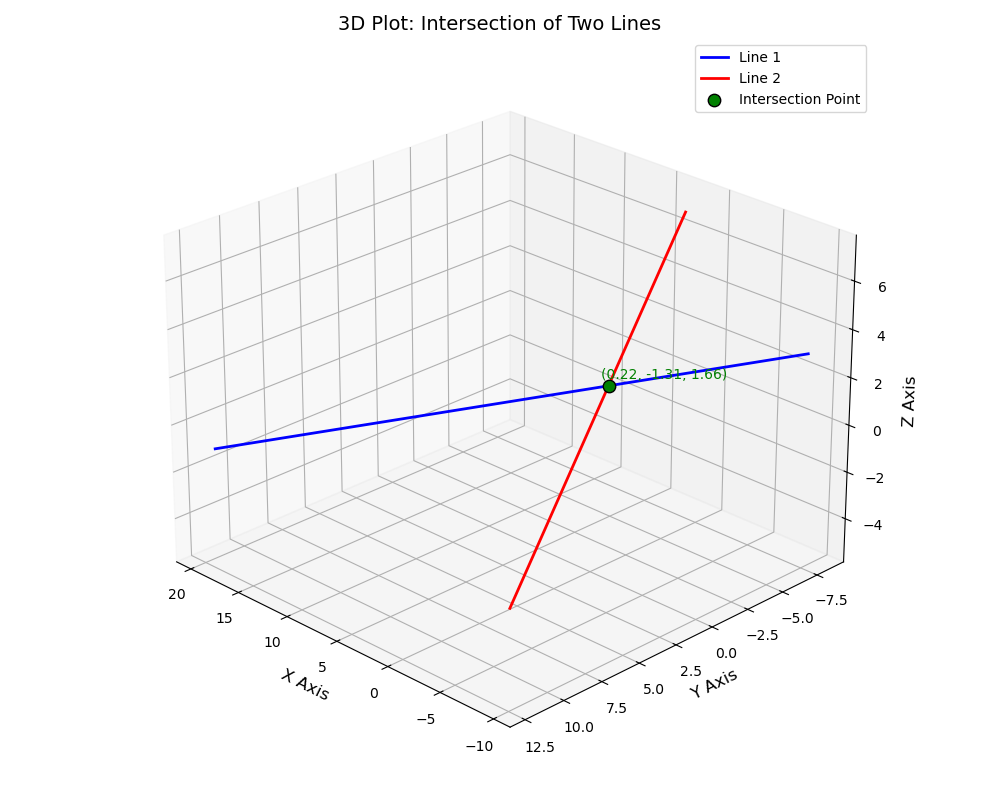
\includegraphics[width=0.9\columnwidth]{figs/fig71.png}
        \caption{}
        \label{fig:placeholder}
    \end{figure}
\end{frame}
\begin{frame}{PLOTS}
    \begin{figure}
        \centering
        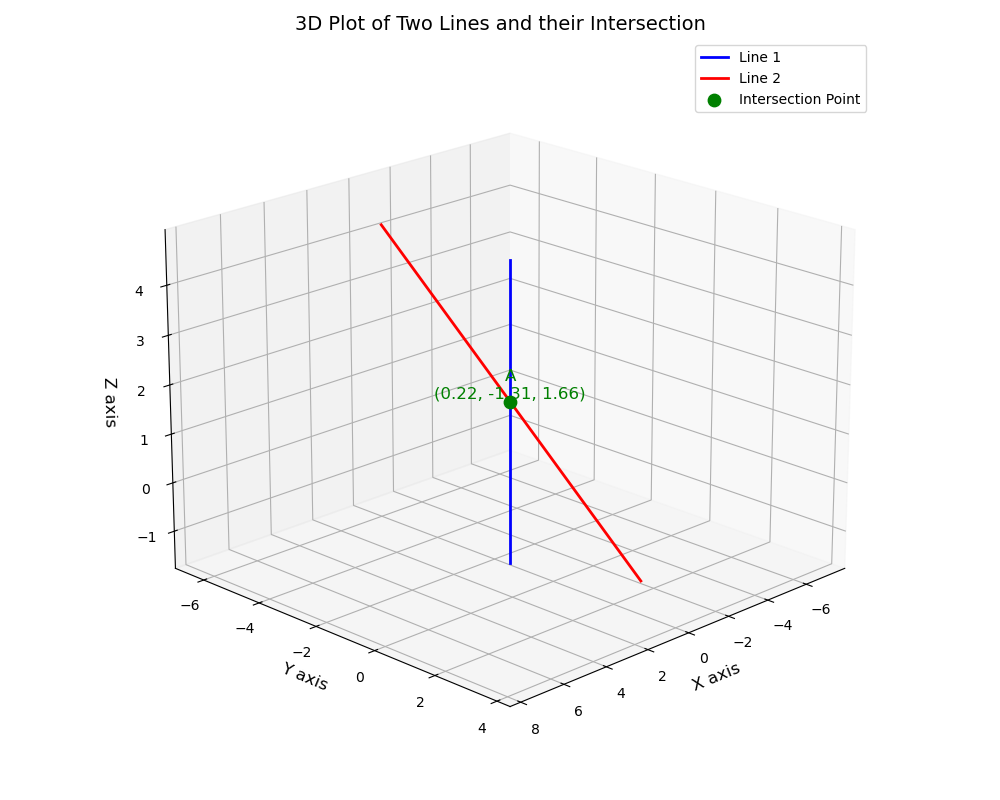
\includegraphics[width=0.9\columnwidth]{figs/fig72.png}
        \caption{}
        \label{fig:placeholder}
    \end{figure}
\end{frame}
\end{document}